Advancements in speech transcription and translation technologies have been propelled by the increasing availability of large-scale datasets. These systems, which underpin applications such as automatic speech recognition (ASR) and automatic speech translation (AST), require extensive and diverse data to achieve high accuracy, robustness, and scalability. The necessity for such data arises from the complexity of human speech, which encompasses a vast range of linguistic, acoustic, and contextual variations.

Despite the growing demand, high-quality human-annotated speech data remains scarce due to the high cost and extensive effort required for curation. Unlike textual data, the availability of human-annotated speech data is significantly constrained, posing challenges for the continued development of speech foundation models. With the rise of large language models (LLMs), substantial computational resources have been allocated to training such systems, and projections suggest that human-generated text annotations may soon become depleted \cite{villalobos2022will}. A similar trend is expected for human-labeled speech data.

However, a vast amount of unlabeled speech data exists online, offering an opportunity to enhance speech models through pseudo-labeling techniques. This is particularly critical for low-resource languages, where manually annotated speech data is even scarcer. By leveraging pseudo-labeled data, ASR and AST systems can be significantly improved for underrepresented languages, mitigating linguistic biases and fostering more inclusive speech technologies.


While pseudo-labeled data is increasingly utilized in speech model training \cite{barrault2023seamless,puvvada2024less}, much of this data remains proprietary. Open-sourcing such datasets would promote transparency, reproducibility, and accessibility in speech research, facilitating broader collaboration between academia and industry. This is particularly important for low-resource languages, where public access to high-quality training data could accelerate the development of more accurate speech models.

Efforts to open-source speech data remain limited. Notable examples include YODAS \cite{li2024yodasyoutubeorienteddatasetaudio} and YouTube-Commons (YTC)
\cite{pleias2025youtube}, which provide large-scale datasets with labels derived from YouTube captions, albeit without guarantees regarding quality or source reliability. More recently, MOSEL \cite{mosel} has released pseudo-generated labels for European languages, covering datasets such as VoxPopuli \cite{wang-etal-2021-voxpopuli} and LibriLight \cite{kahn2020libri}. Other community efforts have highlighted corpus creation pipelines, but these remain restricted to human-generated data and cover only a limited number of languages \cite{chen2021gigaspeechevolvingmultidomainasr}.

Aside from ASR transcripts, open-source projects tackling translation tasks—particularly in speech applications—are exceptionally sparse. Pseudo-label generation for such tasks typically relies on training text-based neural machine translation models to produce automatic speech translation (AST) pairs. However, recent advancements in LLMs have significantly improved their reliability for these tasks.
Motivated by similar effort in text translation \cite{finkelstein-etal-2024-introducing}, we explore the use of open-source LLMs for generating pseudo-labeled translation pairs for speech translation, which is the first to the best of our knowledge.
Our approach builds on prior ASR and AST\cite{barrault2023seamless,puvvada2024less} pseudo-labeling efforts by improving the efficiency of the labeling pipeline, ensuring open-source accessibility, expanding language coverage, and generalizing across diverse corpora. 

To summarize, the main contributions of this work are as follows:  
\begin{itemize}  
    \item Open-source large-scale speech processing pipeline.\footnote{\href{https://github.com/NVIDIA/NeMo-speech-data-processor/tree/main/dataset_configs/multilingual/granary}{\url{https://github.com/NVIDIA/NeMo-speech-data-processor/tree/main/dataset_configs/multilingual/granary}}}
    
    \item Efficient method for generating translation pairs from ASR transcripts across 25 languages.
    \item 643k hours of high-quality pseudo-labeled data for 25 languages.
    \item Evaluation of the quality of pseudo-labeled data against the MOSEL pipeline for both high- and low-resource languages.
\end{itemize}

\begin{figure*}[!ht]
  \centering
  \caption{Granary pseudo-labeling pipeline. The pipeline consists of two parts: ASR and AST. The ASR pipeline includes segmentation, two-pass ASR model inference, language ID verification, text filtering, and Punctuation and Capitalization (PnC) restoration. The AST pipeline involves AST pair generation using the EuroLLM model, followed by Quality Estimation filtering.}
  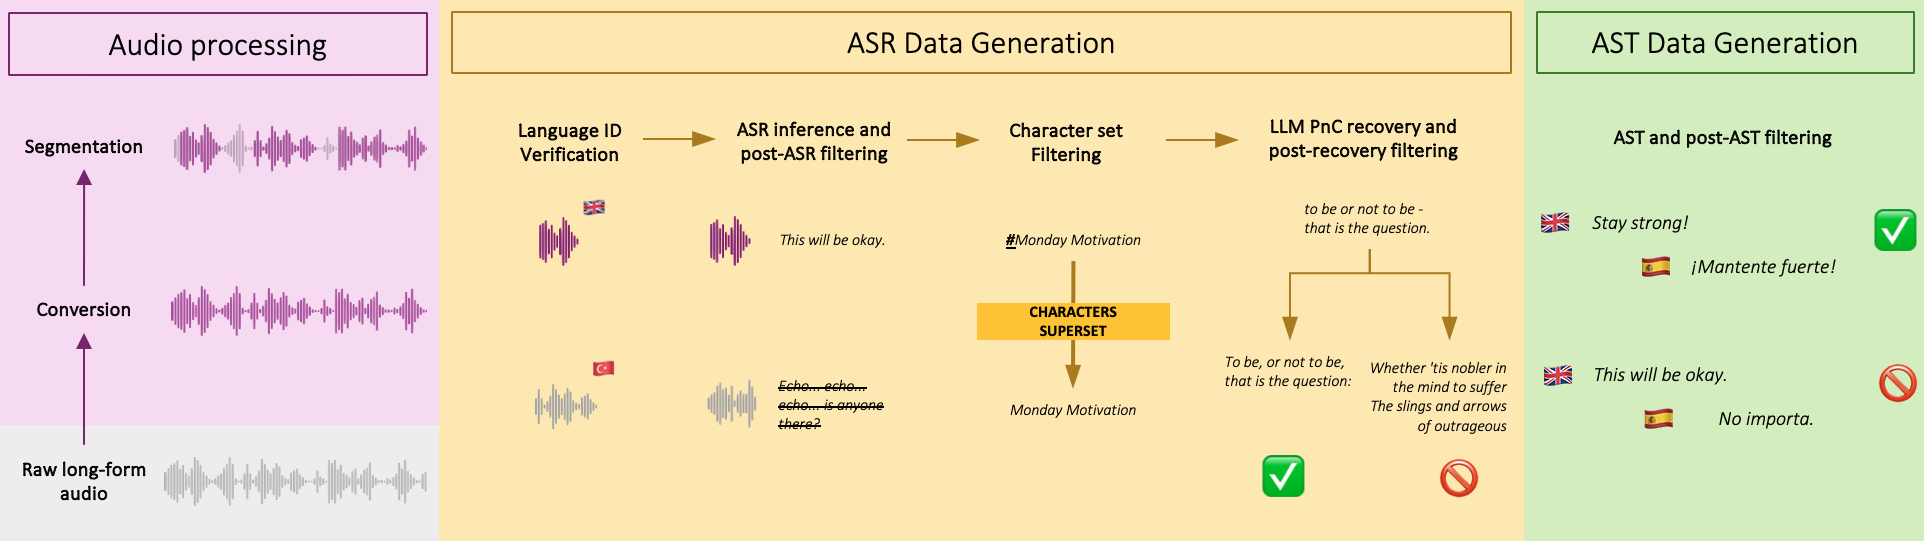
\includegraphics[width=0.88\linewidth]{figures/schema_v4.png}
  \label{fig:speech_production}
\end{figure*}
